%\clearpage
\bibliographystyle{IEEEtran} % We choose the "plain" reference style
\bibliography{relatedworks.bib} % Entries are in the refs.bib file

%  \begin{wrapfigure}{l}{25mm} 
%    %\includegraphics[width=1in,height=1.25in,clip,keepaspectratio]{fig/hamburg-two-drone-dist-graph/two-drone-dist-graph.png}
%  \end{wrapfigure}\par
\setlength{\parskip}{0em}

\begin{IEEEbiography}
[{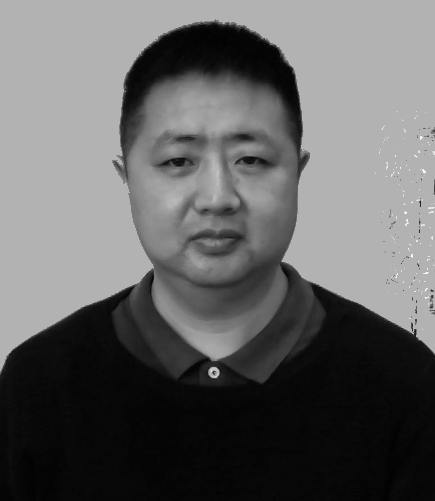
\includegraphics[width=1in,height=1.25in,clip,keepaspectratio]{fig/bio-pics/bio-pic-manduhu.jpg}}]{Manduhu Manduhu}
 received the M.Sc. and Ph.D. degrees
in information engineering from Hiroshima University,
Japan, in 2010 and 2013, respectively.
He is currently a PostDoc researcher at the Drone Systems Lab of the University of the West of Scotland. His research interests include parallel algorithms, physics‑based simulation, and deep learning for object detection and segmentation.
\end{IEEEbiography}


\begin{IEEEbiography}
[{
\includegraphics[width=1in,height=1.25in,clip,keepaspectratio]{fig/bio-pics/bio-pic-alex.png}}]{Alexander Dow}
~received his B.S. in sound engineering and production from Birmingham City University,
Birmingham, UK in 2016 and his M.S. in digital signal and image processing from the 
University of Sussex, Brighton, UK in 2020. He is currently pursuing his Ph.D. in
drone-based computer vision at the University of the West of Scotland,
Lanarkshire, Scotland.
 
He currently works as a Post-Doctoral Research Assistant in the Drone Systems Lab at the University of the West of 
Scotland. His research interests include computer vision, artificial intelligence on embedded systems, LiDAR and hyperspectral imaging.
\end{IEEEbiography}


%\begin{IEEEbiography}
%[{\includegraphics[width=1in,height=1.25in,clip,keepaspectratio]{fig/bio-pics/bio-pic-petar.png}}]{Petar Trslic}
% is a PostDoc researcher at the CRIS of the University of Limerick (UL).
% He received both his BSc and MSc degrees in Mechanical Engineering from the University of Zagreb. 
%Petar finished his PhD at UL in March 2020. During his PhD, he was working on the development of advanced monitoring,
% control systems and onboard robotics for the automation of MRE inspection, repair and maintenance.
%\end{IEEEbiography}

\begin{IEEEbiography}
[{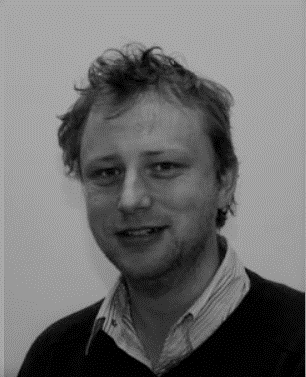
\includegraphics[width=1in,height=1.25in,clip,keepaspectratio]{fig/bio-pics/bio-pic-ger.png}}]{Gerard Dooly}
received the B.Eng. degree from the Electronic and Computer Engineering Department, University of Limerick, in 2003, and the Ph.D. degree from the Optical Fibre Sensors Research Centre, 
University of Limerick, in 2008, on the topic “An Optical Fibre Sensor for the Measurement of Hazardous Emissions from Land Transport Vehicles.”
For over ten years, he has worked extensively in field robotics at UL. His research interests include real-time 3-D reconstruction, machine vision, machine learning, optical fibre sensors, subsea structural health monitoring, 
teleoperation, and automated docking and intervention. He is involved in robotics for harsh environments in offshore setting and is developing systems to address beyond visual line of sight operations for UAS. 
He is focused on the design and development of robotics and has engaged in numerous field operations and survey missions both in Ireland and on the continent. Some of his recent offshore operations involved environmental sensing, 
anti-mine countermeasure ops, remote UAS for incident response, archaeological survey, and hybrid long range UAS technologies.
\end{IEEEbiography}


\begin{IEEEbiography}
[{
\includegraphics[width=1in,height=1.25in,clip,keepaspectratio]{fig/bio-pics/bio-pic-james.png}}]{James Riordan} 
~received the B.Eng. degree in electronic engineering specializing in aircraft simulation
systems and the Ph.D. degree in real-time processing of acoustic signals from the University of
Limerick, Ireland.
 
Currently, he is a Full Professor with the University of the West of Scotland, U.K.,
where he is also the Director of the Drone Systems Laboratory. He is also a Principal Investigator
of multiple research projects funded by European
Commission and U.K. Research and Innovation. His research interests include artificial intelligence,
computer vision, and sensing methods to extend the safe and sustainable
application of autonomous vehicles in land, air, and sea.
\end{IEEEbiography}





